\documentclass[letterpaper, 10 pt]{report}

% For handling graphics
\usepackage{graphicx}
% For multirows in tables
\usepackage{multirow}
% For colors
\usepackage{color}
% For hyperlink
\usepackage{hyperref}
\hypersetup{
    colorlinks,
    linktoc=all,
    citecolor=black,
    filecolor=black,
    linkcolor=black,
    urlcolor=blue
}
\usepackage[margin=1.0in]{geometry}
\usepackage{listings}

\setcounter{secnumdepth}{-2}
% -------------------------------------------------------------------------------------
% TITLE PAGE
% -------------------------------------------------------------------------------------
\begin{document}
\begin{titlepage}
\center
% Headings
\textsc{\LARGE Georgia Institute of Technology}\\[1.5cm]
\textsc{\large Center for Robotics \& Intelligent Machines}\\[0.5cm]
\textsc{\large Humanoid Robotics Lab}\\[0.5cm]
% Title
\rule{\linewidth}{0.5mm}\\[0.4cm]
{\huge \bfseries GT Mission Manual}\\[0.4cm]
\rule{\linewidth}{0.5mm}\\[1.5cm]
% Author
\textsc{\normalsize M.X. Grey}\\
\textsc{\normalsize Eric Huang}\\
\textsc{\normalsize Andrew Price}\\
\textsc{\normalsize Peter Vieira}\\[1.5cm]
% Image
\includegraphics[width=5.0cm]{figures/hubo-titlepage}
% Fill rest of page with whitespace
\vfill
\end{titlepage}


% TABLE OF CONTENTS
% -------------------------------------------------------------------------------------
\tableofcontents
\newpage


% -------------------------------------------------------------------------------------
% CODE REPOS
%
\section{Code Repositories}\label{sec:code-repos}
\subsection{Real-time Code}
Code repositories that run in real-time on the robot.
\begin{itemize}
\item hubo-ach
  \begin{itemize}
	\item \url{https://github.com/hubo/hubo-ach}
	  \begin{itemize}
	    \item Dependencies: \textit{ach, libreadline.}
	  \end{itemize}
  \end{itemize}
\item hubo-motion-rt
	\begin{itemize}
	\item \url{https://github.com/hubo/hubo-motion-rt}
	  \begin{itemize}
	    \item Dependencies: \textit{hubo-ach, RobotKin, urdfdom, eigen3.}
	  \end{itemize}
  \end{itemize}
\item hubomz
  \begin{itemize}
	\item \url{https://github.com/golems/hubomz}
	  \begin{itemize}
	    \item Dependencies: \textit{hubo-ach, hubo-motion-rt, expat, freeglut3.} 
	  \end{itemize}
  \end{itemize}
\end{itemize}
\subsection{ROS Code}
Code repositories that use ros-groovy.
\begin{itemize}
\item hubo\_init : GUI for initializing Hubo and controlling hubo-ach level settings
  \begin{itemize}
	\item \url{https://github.com/hubo/hubo\_init/}
	  \begin{itemize}
	    \item Dependencies: \textit{hubo-ach}
	  \end{itemize}
  \end{itemize}
\item hubo\_walk : GUI for ZMP walk generator
  \begin{itemize}
	\item \url{https://github.com/hubo/hubo\_walk}
	  \begin{itemize}
	    \item Dependencies: \textit{hubo-motion-rt, hubomz}
	  \end{itemize}
  \end{itemize}
\item joystick\_integrator : Converts SpaceNav joystick positions to 3D poses
  \begin{itemize}
    \item \url{https://github.com/a-price/joystick\_integrator}
  \end{itemize}
\item hubo\_motion\_ros : Provides joint-level and end-effector-level teleoperation, MoveIt-based kinematics server, and temporary ROS trajectory executor.
  \begin{itemize}
	\item \url{https://github.com/a-price/hubo\_motion\_ros}
	  \begin{itemize}
	    \item Dependencies: \textit{hubo\_ros\_core, joystick\_integrator, drchubo, ros-groovy-control-msgs, ros-groovy-moveit-msgs}
	  \end{itemize}
  \end{itemize}
\end{itemize}
\newpage

% -------------------------------------------------------------------------------------
% WALL DRILLING INTRO
%
\section{Wall Drilling Task}\label{wall-drilling-task}

\subsection{Procedure}
\begin{enumerate}
\item Identify the drill using robot/human judgement from robot perception feedback.
\item Walk to the drill and pick it up using vision and teleopration from the hubo\_maniupaltion\_planner panel.
\item Identify wall location using human judgement of robot perception.
\item Walk to the wall and face it using the hubo\_walk panel.
\item Begin static balancing using hubo\_walk panel.
\item Use hubo\_manipulation\_planner to identify points on the wall defining polygon to drill out and it's distance away from the wall. Step closer if needed.
\item Send the points in 6-dimensions to the manipulation daemon using the end-effector interpolation mode to drill the object out.
\item Remove drill from wall and place on table or drop.
\end{enumerate}
\begin{figure}[ht]
  \centering
  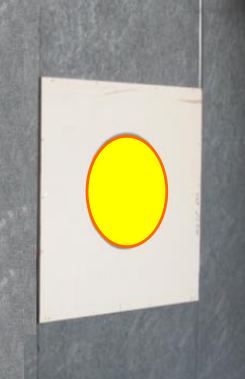
\includegraphics[width=5.0cm]{figures/wall-drilling}
  \caption{Picture of example target to drill out.}
  \label{fig:Wall-image}
\end{figure}

\newpage

% -------------------------------------------------------------------------------------
% RUBBLE CLEARING INTRO
%
\section{Rubble Clearing Task}\label{sec:rubble-clearing-task}
\subsection{Procedure}
\begin{enumerate}
\item Identify the location of the rubble/door using robot/human judgement from robot perception feedback.
\item Walk to the rubble and face it using the hubo\_walk panel.
\item Begin static balancing and squat to height which allows picking up rubble items.
\item Use dual-arm teleoperation to pick up the pieces of rubble and toss them to the side.
\end{enumerate}
\begin{figure}[ht]
  \centering
  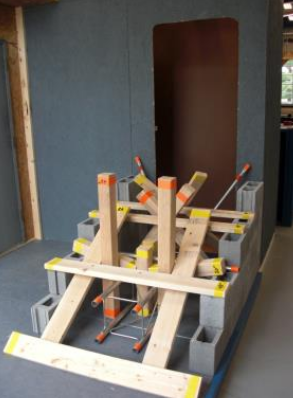
\includegraphics[width=5.0cm]{figures/rubble-clearing}
  \caption{Picture of example rubble scene.}
  \label{fig:Rubble-image}
\end{figure}

\newpage

% -------------------------------------------------------------------------------------
% INSTRUCTIONS
%
\section{Operation Instructions}\label{sec:operating-instructions}
This section details how to operate Hubo from the initialization phase to execution of the tasks. The different phases include \textit{Starting-up Hubo}, \textit{Starting-up Perception}, \textit{Walking}, and \textit{Teleop Manipulation}.
\subsection{Starting-up Hubo}
This section describes how to start-up Hubo.
\begin{enumerate}
  \item ssh hubo@192.168.0.201
  \item Turn on motor controllers with remote
  \item sudo service hubo-motion start
  \item launch RViz
    \begin{itemize}
    	  \item roscore
    	  \item rosrun rviz rviz
    	  \item Click on the \textit{HuboInitPanel} panel tab.
    \end{itemize}
  \begin{figure}[ht]
    \centering
    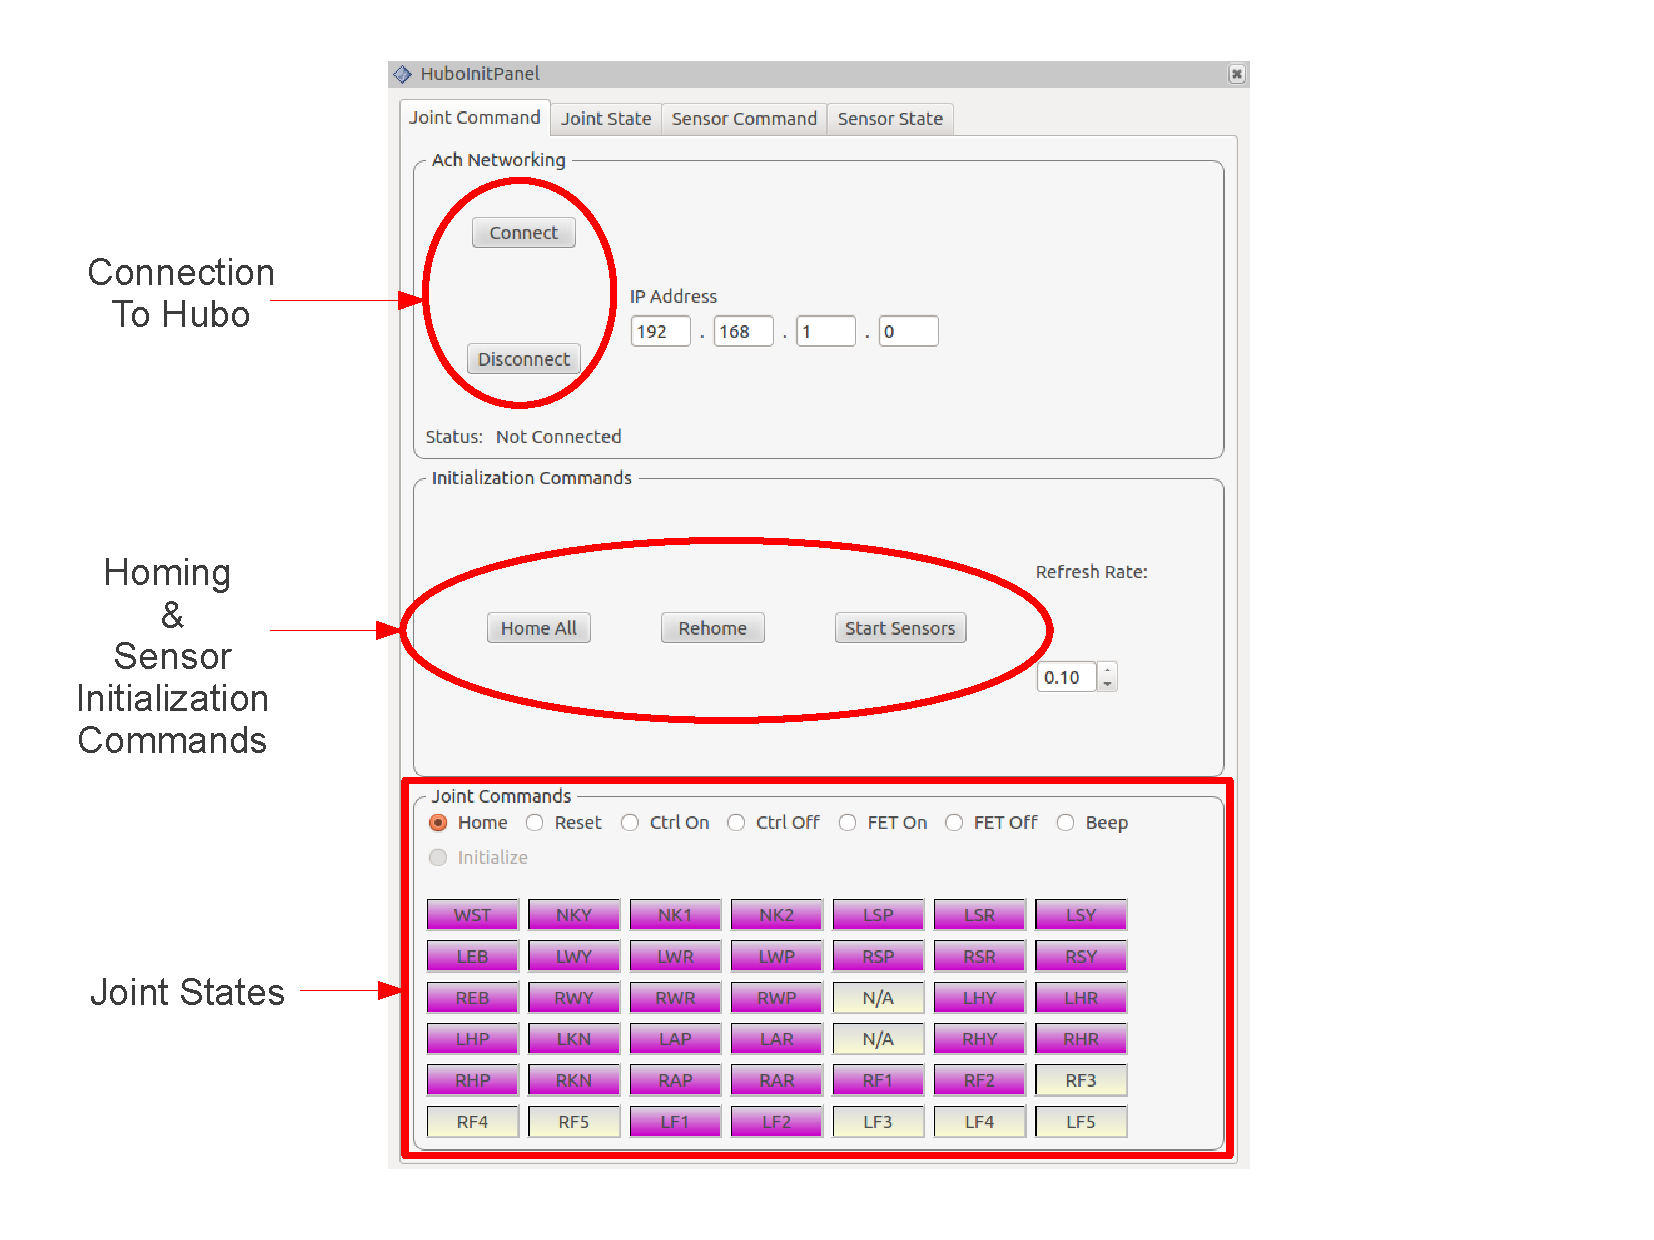
\includegraphics[width=15.0cm]{figures/hubo-init.pdf}
    \caption{Picture of hubo\_init panel.}
    \label{fig:hubo-init-image}
  \end{figure}
  \item Ensure "IP Address" is correct.
  \item Click "Connect" to send and receive ach channels between Hubo's computer and the remote computer. If it won't connect see the Troubleshooting section.
  \item Click "Home All" to home all of Hubo's joints, if not on the ground and not homed. If already homed and standing, continue skip to step.
  \item If any active joints do not home, indicated by the color in the \textit{Joint State} section not being gray, click the "Rehome". Button color meanings are
    \begin{itemize}
      \item GRAY: homed
      \item PURPLE: not homed
      \item RED: error
      \item WHITE: inactive
    \end{itemize}
  \item If any joints won't home, you can do one of two options:
    \begin{enumerate}
      \item Run sudo service hubo-motion stop, run sudo servi	ce hubo-motion start, and then start the process over again.
      \item Click the \textit{Reset} radio button and then click the joint(s) that won't home. Then click the \textit{Home} radio button and click the joint(s) that didn't home. Then press the "Rehome" button again.
    \end{enumerate}
  \item Once the joints are all homed, press the "Start Sensors" button to initialize the IMU and Force/Torque sensors.
  \item Click on the \textit{Sensor State} tab and ensure the sensor values are updating and are reasonable. If they aren't, then restart the whole process.
\end{enumerate}

\subsection{Starting-up Perception} \label{sec:starting-up-perception}
This section is heavily under construction. Generally, what you will need to do is probably something like this:
  \begin{lstlisting}[language=bash]
    $ roslaunch openni2_launch openni2.launch
  \end{lstlisting}
Or, hopefully when everything gets straightened out, it will be like:
  \begin{lstlisting}[language=bash]
    $ roslaunch hubo_vision_common full.launch
  \end{lstlisting}

\subsection{Walking}
This section describes how to make Hubo walk. And assumes the robot is already up and running and standing on the ground on two feet.
  \begin{enumerate}
    \item Click on the \textit{HuboWalkPanel} tab.
    \begin{figure}[ht]
      \centering
      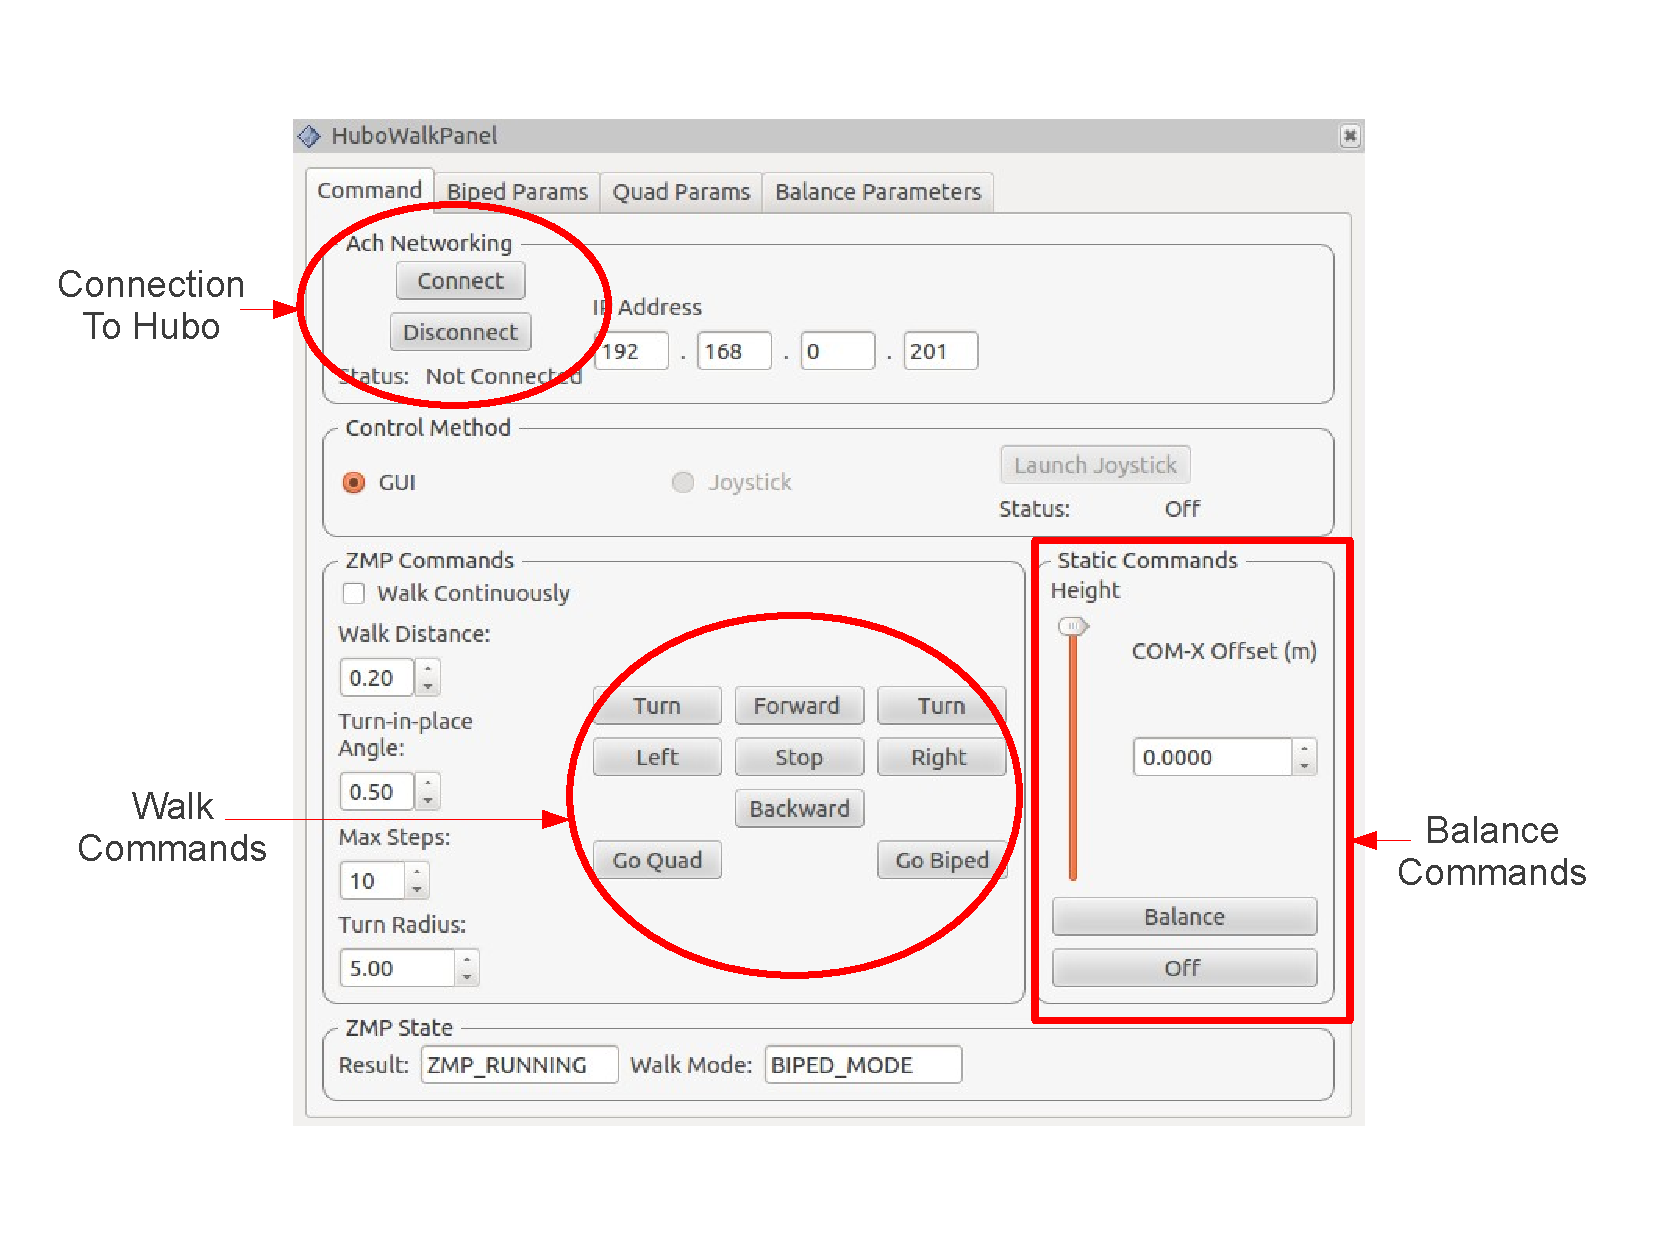
\includegraphics[width=15.0cm]{figures/hubo-walk.pdf}
      \caption{Picture of hubo\_walk panel.}
      \label{fig:hubo-walk-image}
    \end{figure}
    \item Ensure the IP Address is correct.
    \item Click "Connect" to send and receive ach channels between Hubo's computer and the remote computer. If it won't connect see the Troubleshooting section.
    \item Click the \textit{Joystick} radio button if it is not already selected.
    \item Based on vision feedback enter desired walk distance, max number of steps, and turn-in-place angle (for turning in place).
    \item Click the "Go Quad" button to transition into quadruped mode.
    \item Click the walk command desired to get to your desired goal. (Eventually the interface will use a desired location and orientation, and the ZMP walk generator will create a footstep plan to get there.) The \textit{Walk Continuously} checkbox determines whether or not to walk the specified distance or walk until receiving a stop command. The \textit{ZMP State} section at the bottom of the panel display the state of the ZMP walker generator.
    \item Click "Go Biped" to get back up on two feet in order to manipulate objects.
    \item In the \textit{Balance Commands} section of the panel, click "Balance" to go into static balancing mode.
    \item The x-location of the center of mass can be adjusted in the \textit{COM-X Offset (m)} field. Then click the "Balance" button to send the command.
    \item The squat height of the robot can be adjusted by sliding the \textit{Height} slider up and down, which automatically sends the command to the robot.
  \end{enumerate}

\subsection{Manipulation}
This section describes how to teleoperate Hubo in order to dual-arm manipulate objects in the environment.
NB: First install all software outlined in \nameref{sec:code-repos}
\begin{enumerate}
  \item If you haven't already, start up ROS
    \begin{lstlisting}[language=bash]
  		$ roscore
  		$ rosrun rviz rviz
	\end{lstlisting}
  \item Start the teleoperation interface
    \begin{lstlisting}[language=bash]
  		$ roslaunch hubo_motion_ros fullbody_teleop.launch
	\end{lstlisting}
  \item (Optional) Start up the Vision package by following the instructions in \nameref{sec:starting-up-perception}.
\end{enumerate}
  \begin{figure}[ht]
    \centering
    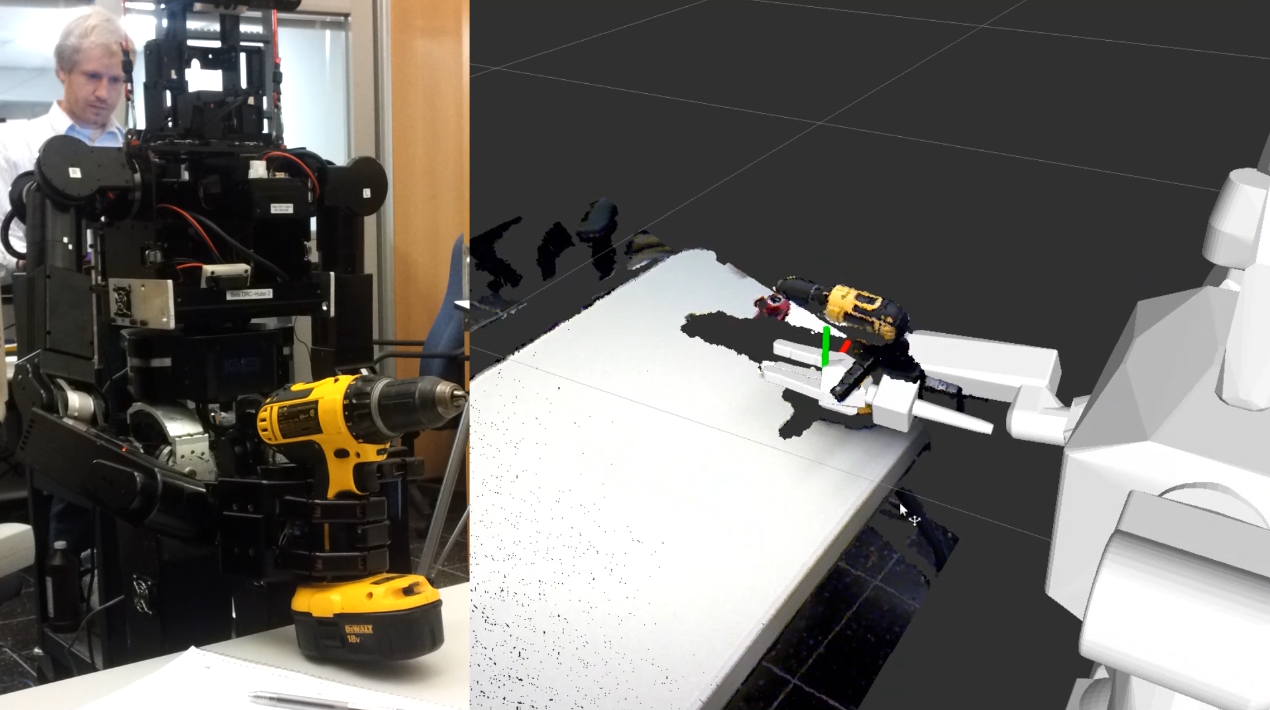
\includegraphics[width=12.0cm]{figures/pickup-drill-rviz}
    \caption{Picture of teleoperation of picking up a drill.}
    \label{fig:pickup-drill-rviz-image}
  \end{figure}
  \begin{figure}[ht]
    \centering
    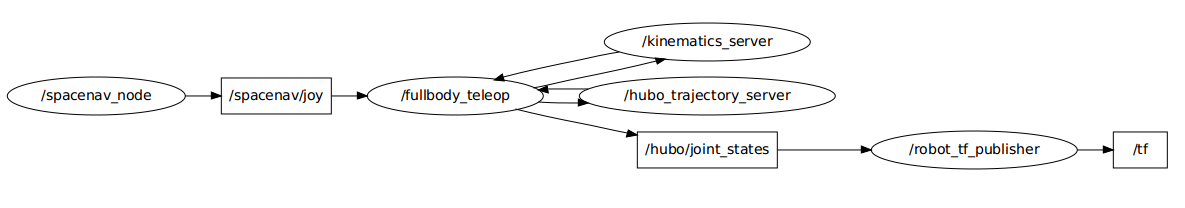
\includegraphics[width=12.0cm]{figures/teleop-rosgraph}
    \caption{Simplified ROS Graph created by fullbody\_teleop.launch.}
    \label{fig:teleop-rosgraph-image}
  \end{figure}


% -------------------------------------------------------------------------------------
% TROUBLESHOOTING
%
\clearpage
\section{Troubleshooting}\label{sec:troubleshooting}
\begin{table}[ht]
  \centering
  \caption{Troubleshooting Table}
  \begin{tabular}{|p{4.5cm}|p{4.5cm}|p{4.5cm}|} \hline
    \multicolumn{1}{|c|}{Symptom} & \multicolumn{1}{|c|}{Causes} & \multicolumn{1}{|c|}{Solution} \\ \hline
    Can't ssh to Hubo's PC & Not on correct network. \newline Hubo's PC is stuck in the Grub menu & Connect to the correct network. \newline Connect a monitor and keyboard to Hubo's PC and debug, or just a keyboard and press enter. \\
    \hline
    Can't connect to the robot in RViz panel & Not on the correct network. \newline The daemons are not running on Hubo & Connect to the correct network. \newline Ensure daemons are running by typing \textit{ps aux $|$ grep daemon} or restarting Hubo and running \textit{sudo service hubo-motion start}.  \\
    \hline
    Receiving ACH\_OVERFLOW from rviz command. \newline HuboInitPanel joint names don't showing up correctly. & Don't have matching or most up-to-date installs of hubo-ach, hubo-motion-rt, hubomz or possible another repo. & Make sure your on the right branch in each repo and reinstall on both machines. \\
    \hline
    Robot homes only the upper or lower body, or neither. & CAN line got corrupted. & Shutdown and turn off the Hubo PC and turn it back on and try again. \\
    \hline
  \end{tabular} \label{tbl:troubleshooting}
\end{table}


% -------------------------------------------------------------------------------------
% REFERENCES
% -------------------------------------------------------------------------------------
%\bibliography{}

% -------------------------------------------------------------------------------------
% END DOCUMENT
% -------------------------------------------------------------------------------------
\end{document}
